\chapter{Relativistic Dynamics}\label{ch:b3:relativistic-dynamics}

In 1964 William Bertozzi filmed electrons racing down a linear
accelerator: each burst was given a measured energy, and its speed was
clocked over \qty{8.4}{m} of flight. Newton predicted that
\qty{15}{MeV} electrons should fly at eight times the speed of light;
the stopwatch said $0.9999c$ and refused to go further, however hard
the electrons were pushed. Kinematics told us in the last chapter that
$c$ is a limit; dynamics must now explain what happens to the pushing
--- where the work goes when speed no longer grows. The answer
reorganises mechanics around a new momentum and a new energy, joined
in the most famous equation in physics: energy stored is mass, mass is
energy in residence, $E = mc^2$. This chapter builds the dynamics,
then puts it to work where it lives daily --- radioactive decays,
particle collisions, and the accelerators that turn motion into new
matter.

\section{Momentum and energy, rebuilt}

\begin{remark}[Why $m\vect v$ had to go]\label{rem:b3:relativistic-dynamics:why}
Classical momentum $m\vect v$ is conserved in every frame \emph{if}
velocities transform à la Galileo. They do not
(\cref{prop:b3:relativistic-kinematics:addition}): a collision that
conserves $\sum m\vect v$ in one frame fails to in another, so the
old momentum cannot be a law of nature --- at best a slow-speed
shadow of one. The repair is to measure the velocity with the
particle's \emph{own} clock: $\dd\vect r/\dd\tau =
\gamma\,\vect v$ transforms cleanly, and $m\,\dd\vect r/\dd\tau$
turns out to be conserved in all frames at once.
\end{remark}

\begin{definition}[Relativistic momentum and energy]\label{def:b3:relativistic-dynamics:momentum-energy}
\index{relativistic momentum}\index{relativistic energy}\index{rest energy}
A particle of mass $m$ and velocity $\vect v$ ($\gamma = 1/\sqrt{1 -
v^2/c^2}$) carries the momentum and the energy
\[
\vect p = \gamma m\vect v , \qquad
E = \gamma mc^2 .
\]
At rest, $E_0 = mc^2$: the \emph{rest energy}. The kinetic energy is
what motion adds, $E_k = E - mc^2 = (\gamma - 1)mc^2$, which for $v
\ll c$ reduces to the familiar $\tfrac12 mv^2$ (expand $\gamma$). In
every isolated process, total $\vect p$ and total $E$ --- rest
energies included --- are conserved.
\end{definition}

\begin{theorem}[The energy--momentum relation]\label{thm:b3:relativistic-dynamics:relation}
\index{energy--momentum relation}
For any particle,
\[
E^2 = (pc)^2 + (mc^2)^2 ,
\qquad
\vect v = \frac{\vect p\,c^2}{E} :
\]
the combination $E^2 - p^2c^2 = m^2c^4$ has the same value in every
frame --- it is to energy and momentum what the interval is to time
and space. Two regimes: at low speed, $E \approx mc^2 + p^2/2m$; at
high energy ($E \gg mc^2$), $E \approx pc$ and $v \to c$: pushing
harder adds energy and momentum, almost no speed.
\end{theorem}

\begin{proof}
$E^2 - p^2c^2 = \gamma^2m^2c^4(1 - v^2/c^2) = m^2c^4$; and $pc^2/E =
\gamma mvc^2/\gamma mc^2 = v$. Frame invariance follows because $m$
and $c$ are frame-independent.
\end{proof}

\begin{proposition}[Massless particles]\label{prop:b3:relativistic-dynamics:massless}
\index{photon!momentum}
A particle of zero mass has $E = pc$ and moves at exactly $c$ in every
frame; it cannot be slowed, only redshifted. The photon is the
standard case: $E = h\nu$ and $p = h\nu/c = h/\lambda$ --- the
Planck--Einstein relations of the Year 1 volume, now seen as the
$m = 0$ corner of mechanics.
\end{proposition}

\begin{proof}
Set $m = 0$ in \cref{thm:b3:relativistic-dynamics:relation}: $E = pc$
and $v = pc^2/E = c$.
\end{proof}

\begin{omfigure}
\begin{tikzpicture}
  \begin{axis}[omaxis, axis x line=bottom, axis y line=left,
    width=6.6cm, height=5.4cm, xmin=0, xmax=4.3, ymin=0, ymax=1.35,
    xlabel={$E_k/mc^2$}, ylabel={$v^2/c^2$},
    xlabel style={at={(axis description cs:0.5,-0.1)}, anchor=north},
    xtick={1,2,3,4}, ytick={0.5,1}, clip=false]
    \addplot[omExo, dashed, thick, domain=0:0.68] {2*x};
    \addplot[omDef, very thick, domain=0:4.3, samples=80] {1 - 1/(1+x)^2};
    \addplot[gray, dashed, domain=0:4.3] {1};
    \node[omExo, font=\scriptsize, anchor=west] at (axis cs:0.8,1.24) {Newton: $v^2 = 2E_k/m$};
    \node[omDef, font=\scriptsize, anchor=west] at (axis cs:2.0,0.82) {relativity};
    \fill[omThm] (axis cs:0.87,0.714) circle (1.6pt);
    \fill[omThm] (axis cs:1.96,0.886) circle (1.6pt);
    \fill[omThm] (axis cs:2.94,0.935) circle (1.6pt);
  \end{axis}
  \begin{axis}[omaxis, axis x line=bottom, axis y line=left,
    width=6.6cm, height=5.4cm, xmin=0, xmax=3, ymin=0, ymax=3.3,
    xshift=7.2cm,
    xlabel={$pc/mc^2$}, ylabel={$E/mc^2$},
    xlabel style={at={(axis description cs:0.5,-0.1)}, anchor=north},
    xtick={1,2,3}, ytick={1,2,3}, clip=false]
    \addplot[omDef, very thick, domain=0:3, samples=60] {sqrt(1+x*x)};
    \addplot[omExo, dashed, domain=0:3] {x};
    \draw[<->, omThm] (axis cs:0,0.04) -- (axis cs:0,0.96);
    \node[omThm, font=\scriptsize, anchor=west] at (axis cs:0.06,0.5) {$mc^2$};
    \node[omExo, font=\scriptsize, anchor=north west] at (axis cs:2.1,2.0) {$E = pc$ (light)};
    \node[omDef, font=\scriptsize, anchor=south east] at (axis cs:2.9,3.1) {$E = \sqrt{p^2c^2 + m^2c^4}$};
  \end{axis}
\end{tikzpicture}

{\small Left: Bertozzi's ``ultimate speed'' experiment --- measured
electron speeds (dots) follow the relativistic curve and saturate at
$c$ while Newton's line sails past it. Right: the energy--momentum
hyperbola; its offset at $p = 0$ is the \omterm{def:b3:relativistic-dynamics:momentum-energy}{rest energy}, its asymptote the
photon's $E = pc$.}
\end{omfigure}

\begin{example}[Orders of magnitude]\label{ex:b3:relativistic-dynamics:orders}
Particle physics counts energy in electronvolts and masses in
$\unit{MeV}/c^2$: electron $0.511$, proton $938.3$, muon $105.7$, pion
$139.6$. An electron of kinetic energy \qty{1}{MeV} has $\gamma =
2.96$ and $v = 0.94c$ --- already fully relativistic, which is why
electronics stays classical (\unit{eV}) and nuclear physics does not
(\unit{MeV}). A \qty{6.8}{TeV} LHC proton has $\gamma = 7250$ and
trails a photon by only \qty{2.9}{m/s}.
\end{example}

\section{Mass is energy in residence}

\begin{theorem}[Mass--energy equivalence]\label{thm:b3:relativistic-dynamics:emc2}
\index{mass--energy equivalence}\index{mass defect}
The mass of a body is the total energy of its contents, divided by
$c^2$, measured in its rest frame: heat a body, wind its spring,
excite its atoms, and it weighs more by $\Delta E/c^2$; bind its parts
together and it weighs \emph{less} by the binding energy over $c^2$
--- the \emph{\omterm{thm:b3:relativistic-dynamics:emc2}{mass defect}}. Conversely, \omterm{def:b3:relativistic-dynamics:momentum-energy}{rest energy} can be released:
whenever the final masses total less than the initial ones, the
difference $\Delta m\,c^2$ emerges as kinetic energy or radiation.
\end{theorem}
\admitted

\begin{example}[The ledger of $c^2$]\label{ex:b3:relativistic-dynamics:ledger}
$c^2 = \qty{9e16}{J/kg}$: one gram of mass difference is
\qty{9e13}{J}, the energy of a small city for a day. Chemical bonds
(a few eV per molecule) shift masses by parts in $10^{10}$ ---
forever unweighable, which is why chemistry never noticed. Nuclear
binding shifts them by nearly $1\%$: helium weighs $0.7\%$ less than
its four hydrogen ingredients, and that missing fraction, streaming
from the Sun as light, costs it $\Delta m = L_\odot/c^2 =
\qty{4.3e9}{kg}$ every second --- four million tonnes of sunshine.
Annihilation settles the whole account: an electron meeting a
positron leaves nothing but two photons of \qty{511}{keV} each, the
signal by which PET scanners watch a living brain.
\end{example}

\begin{remark}[What ``conversion'' means]\label{rem:b3:relativistic-dynamics:conversion}
Nothing material ``turns into'' energy: total energy was conserved all
along. What changes is its \emph{residence} --- from \omterm{def:b3:relativistic-dynamics:momentum-energy}{rest energy},
which weighs, to kinetic energy and radiation, which fly. The deep
statement of $E = mc^2$ is that inertia itself is an energy content:
a box of hot gas resists acceleration more than the same box cold.
\end{remark}

\section{Collisions and decays}

\begin{definition}[Four-momentum and invariant mass]\label{def:b3:relativistic-dynamics:four-momentum}
\index{four-momentum}\index{invariant mass}
Bundle a particle's energy and momentum into its \emph{four-momentum}
$P = (E/c, \vect p)$. For a system of particles, sum componentwise:
$E_{\text{tot}} = \sum E_i$, $\vect p_{\text{tot}} = \sum\vect p_i$.
The system's \emph{invariant mass} $M$ is defined by
\[
M^2c^4 = E_{\text{tot}}^2 - \|\vect p_{\text{tot}}\|^2c^2 :
\]
the same number in every frame, equal to the total energy (over
$c^2$) in the \emph{centre-of-momentum frame} where
$\vect p_{\text{tot}} = \vect 0$. Note that $M$ exceeds the sum of
the parts' masses whenever they move relative to each other --- two
photons flying apart have $M > 0$ though each is massless.
\end{definition}

\begin{method}[Solving a relativistic collision]\label{met:b3:relativistic-dynamics:method}
(1) Write \omterm{def:b3:relativistic-dynamics:four-momentum}{four-momentum} conservation: $E$ and $\vect p$ together,
never one alone. (2) Compute the invariant $E^2 - p^2c^2$ of
whatever bundle is convenient --- it can be evaluated in the easiest
frame and used in any other. (3) Thresholds: a reaction is possible
when the \omterm{def:b3:relativistic-dynamics:four-momentum}{invariant mass} of the initial state reaches the summed rest
masses of the final one. (4) Decays at rest: momenta of the products
are opposite and equal; energies follow from the masses alone. (5)
Only at the very end, if asked, convert to speeds via $v = pc^2/E$.
\end{method}

\begin{example}[The pion's fingerprint]\label{ex:b3:relativistic-dynamics:pion}
A charged pion at rest decays, $\pi^+ \to \mu^+ + \nu$ (the neutrino
effectively massless). Momentum conservation makes the products
back-to-back with equal $p$; energy conservation reads $m_\pi c^2 =
\sqrt{p^2c^2 + m_\mu^2c^4} + pc$. Solving:
\[
pc = \frac{(m_\pi^2 - m_\mu^2)c^2}{2m_\pi} = \qty{29.8}{MeV} ,
\]
so every muon from a pion decaying at rest is born with exactly
\qty{4.1}{MeV} of kinetic energy --- a monoenergetic line, and its
observation (Powell, 1947) is how the pion's mass was first weighed.
Two-body decays always produce such lines; three-body decays smear
them into spectra, which is precisely how the neutrino was first
suspected in nuclear $\beta$ decay.
\end{example}

\begin{proposition}[Thresholds: the tyranny of the fixed target]\label{prop:b3:relativistic-dynamics:threshold}
\index{threshold energy}\index{collider}
To create new particles, only the \emph{centre-of-momentum} energy
$Mc^2$ is available. A beam of energy $E$ striking a target of mass
$m_{\text{t}}$ at rest yields
\[
M^2c^4 = m_{\text{b}}^2c^4 + m_{\text{t}}^2c^4 +
2\,E\,m_{\text{t}}c^2 :
\]
the useful energy grows only as $\sqrt E$ --- the rest is wasted on
pushing the debris forward. Two identical beams colliding head-on
yield $Mc^2 = 2E$: all of it useful. This single formula is why the
frontier machines are colliders
(\cref{pb:b3:relativistic-dynamics:1}).
\end{proposition}

\begin{proof}
Evaluate $E_{\text{tot}}^2 - p_{\text{tot}}^2c^2$ in the lab:
$(E + m_{\text{t}}c^2)^2 - p^2c^2$ with $p$ the beam momentum; expand
and use $E^2 - p^2c^2 = m_{\text{b}}^2c^4$. For the collider,
$\vect p_{\text{tot}} = \vect 0$ and $Mc^2 = E_{\text{tot}}$.
\end{proof}

\begin{omfigure}
\begin{tikzpicture}[font=\small, >=Stealth]
  % fixed target
  \begin{scope}
    \fill[omDef] (0,0) circle (2.6pt);
    \draw[->, omDef, very thick] (0.15,0) -- (1.45,0);
    \node[font=\footnotesize] at (0.0,0.42) {$E$};
    \fill[omExo] (2.3,0) circle (2.6pt);
    \node[font=\footnotesize] at (2.3,0.42) {at rest};
    \draw[->, thick] (3.1,0) -- (3.8,0);
    \fill[gray] (4.6,0) circle (2.6pt);
    \draw[->, gray, very thick] (4.75,0) -- (5.9,0);
    \draw[->, gray, thick] (4.68,0.12) -- (5.5,0.62);
    \draw[->, gray, thick] (4.68,-0.12) -- (5.5,-0.62);
    \node[align=center, font=\footnotesize] at (2.9,-1.25)
      {fixed target: $Mc^2 \approx \sqrt{2\,E\,m_{\text{t}}c^2}$\\the debris keeps most of the energy};
  \end{scope}
  % collider
  \begin{scope}[xshift=8.3cm]
    \fill[omDef] (0,0) circle (2.6pt);
    \draw[->, omDef, very thick] (0.15,0) -- (1.45,0);
    \node[font=\footnotesize] at (0.0,0.42) {$E$};
    \fill[omThm] (3.4,0) circle (2.6pt);
    \draw[->, omThm, very thick] (3.25,0) -- (1.95,0);
    \node[font=\footnotesize] at (3.4,0.42) {$E$};
    \node[align=center, font=\footnotesize] at (1.7,-1.25)
      {collider: $Mc^2 = 2E$\\every joule is available};
  \end{scope}
\end{tikzpicture}

{\small Making matter from motion: on a fixed target, momentum
conservation forces the products to keep flying, and the useful
centre-of-momentum energy grows only as $\sqrt E$; in a head-on
collision it is all of $2E$.}
\end{omfigure}

\section{Force and the machines}

\begin{proposition}[Relativistic equation of motion]\label{prop:b3:relativistic-dynamics:force}
\index{synchrotron}
Newton's law survives in the form
\[
\vect F = \frac{\dd\vect p}{\dd t} = \frac{\dd(\gamma m\vect v)}
{\dd t} , \qquad
\frac{\dd E}{\dd t} = \vect F\cdot\vect v .
\]
A magnetic field, forever perpendicular to $\vect v$, changes no
energy and bends the trajectory into a circle of radius
\[
r = \frac{p}{qB}
\]
--- the same formula as in the Year 1 volume, with the relativistic
$p$. But the circulation frequency $qB/\gamma m$ now \emph{falls} as
the particle gains energy: the cyclotron's fixed-frequency push slips
out of step near the MeV scale, and the high-energy machines --- the
\emph{synchrotrons} --- instead ramp their field and their frequency
in synchrony with $\gamma$, holding the beam on one ring.
\end{proposition}

\begin{proof}[Partial proof]
The force law is the definition of dynamics consistent with the new
momentum ($\dd E/\dd t$ follows from
$E^2 = p^2c^2 + m^2c^4$: $E\,\dot E = c^2\vect p\cdot\dot{\vect p}$).
For the circle: $|\dd\vect p/\dd t| = qvB$ with $|\vect p|$ constant
means the momentum vector turns at rate $qvB/p$, so the radius is
$v/(qvB/p) = p/qB$.
\end{proof}

\begin{example}[Reading the LHC like an exercise]\label{ex:b3:relativistic-dynamics:lhc}
Protons of $E = \qty{6.8}{TeV}$ in dipoles of $B = \qty{8.3}{T}$:
$p \approx E/c$ (ultrarelativistic), so $r = p/qB =
\qty{2.7}{km}$ --- and indeed the ring's magnetic bending radius is
\qty{2.8}{km}, the \qty{27}{km} circumference being mostly magnets.
Head-on collisions provide $Mc^2 = \qty{13.6}{TeV}$; to reach that on
a fixed target would take a beam of $2E^2/m_{\text{p}}c^2 \approx
\qty{e17}{eV}$ --- a hundred-fold the reach of any machine ever
built. The collider formula, not stronger magnets, is what bought
the modern energy frontier.
\end{example}

\begin{omfigure}
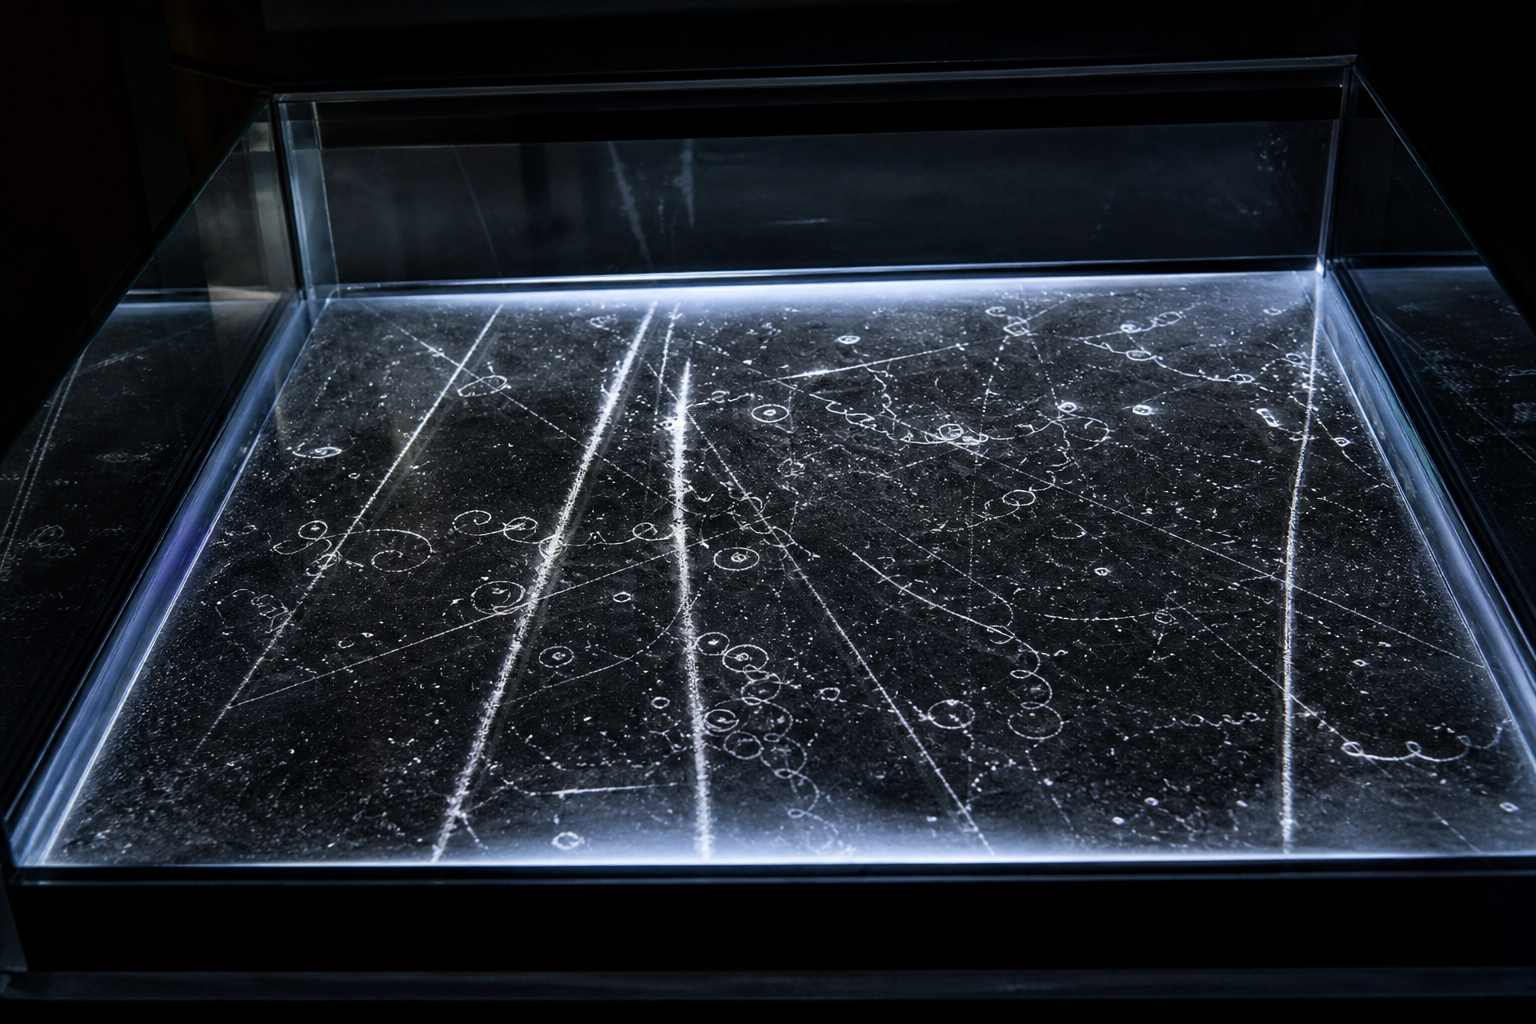
\includegraphics[width=0.58\linewidth]{images/book5/ai/b5-05-cloud-chamber.png}

{\small Charged particles crossing a cloud chamber. Tracks like these --- curling in magnetic fields, appearing in pairs --- turned $E = mc^2$ from a formula into daily bookkeeping: the positron was discovered on such a photograph.}
\end{omfigure}

\section{Exercises}

\begin{exercise}[$\star$]\label{exo:b3:relativistic-dynamics:1}
An electron ($mc^2 = \qty{0.511}{MeV}$) moves at $0.99c$. Compute
$\gamma$, its momentum in $\unit{MeV}/c$, its total and kinetic
energies. Same questions for a proton ($mc^2 = \qty{938}{MeV}$) of
kinetic energy \qty{1}{GeV}.
\end{exercise}

\begin{exercise}[$\star$]\label{exo:b3:relativistic-dynamics:2}
(a) How much energy sleeps in one gram of matter? (b) The Hiroshima
explosion released about \qty{6e13}{J}: what mass difference is that?
(c) The Sun radiates $L = \qty{3.8e26}{W}$: how much mass does it
shed per second, and what fraction of its $\qty{2e30}{kg}$ in ten
billion years? (d) Your phone battery stores \qty{5e4}{J}: by how
much is a charged phone heavier?
\end{exercise}

\begin{exercise}[$\star$]\label{exo:b3:relativistic-dynamics:3}
(a) What momentum does a \qty{5}{mW} laser pointer's beam carry per
second, and what force does the pointer feel? (b) What force does
sunlight (\qty{1.4}{kW/m^2}) exert on a perfectly reflecting
\qty{100}{m^2} solar sail? (c) From rest, how fast is a \qty{10}{kg}
sail-craft moving after a month? (d) Why does a comet's dust tail
point away from the Sun?
\end{exercise}

\begin{exercise}[$\star$]\label{exo:b3:relativistic-dynamics:4}
Practice with units. (a) Show that $\unit{MeV}/c^2$ is a mass unit
and convert the electron mass to kilograms. (b) What is
\qty{1}{GeV/c} in $\unit{kg.m/s}$? (c) An \omterm{def:b3:relativistic-dynamics:four-momentum}{invariant mass} squared
comes out as $s = \qty{16}{GeV^2}$ (in $c = 1$ units): what
centre-of-momentum energy is that? (d) Why do particle physicists set
$c = 1$, and what must a reader re-insert to get SI numbers?
\end{exercise}

\begin{exercise}[$\star\star$]\label{exo:b3:relativistic-dynamics:5}
Bertozzi's electrons had kinetic energies $0.5$, $1$, $4.5$ and
\qty{15}{MeV}. (a) Compute Newton's prediction $v^2 = 2E_k/m$ for
each, in units of $c^2$. (b) Compute the relativistic $v^2/c^2$. (c)
His time-of-flight over \qty{8.4}{m} at \qty{15}{MeV}: what did the
clock read, and what would Newton have predicted? (d) The electrons'
energy was also measured calorimetrically --- by their heat on
impact: why was that step the experiment's real point?
\end{exercise}

\begin{exercise}[$\star\star$]\label{exo:b3:relativistic-dynamics:6}
The charged pion decays at rest: $\pi^+ \to \mu^+\nu$, $m_\pi c^2 =
\qty{139.6}{MeV}$, $m_\mu c^2 = \qty{105.7}{MeV}$, $m_\nu \approx 0$.
(a) Show $pc = (m_\pi^2 - m_\mu^2)c^4/2m_\pi c^2$ and evaluate it.
(b) The muon's kinetic energy and speed. (c) The neutrino's energy.
(d) In flight at $\gamma_\pi = 50$, what are the maximum and minimum
lab energies of the decay muon (decay forward and backward)?
\end{exercise}

\begin{exercise}[$\star\star$]\label{exo:b3:relativistic-dynamics:7}
\omterm{def:b3:relativistic-dynamics:four-momentum}{Invariant mass} in \omterm{def:b3:lagrangian-mechanics:action}{action}. (a) Two photons of \qty{200}{MeV} each fly
at $60^\circ$ to one another: compute the \omterm{def:b3:relativistic-dynamics:four-momentum}{invariant mass} of the pair.
(b) A neutral pion ($m_{\pi^0}c^2 = \qty{135}{MeV}$) decays into two
photons: what is the \omterm{def:b3:relativistic-dynamics:four-momentum}{invariant mass} of the photon pair, in every
frame? (c) Explain how an experiment ``discovers'' a particle as a
bump in the invariant-mass distribution of its decay products. (d)
Two photons of equal energy fly exactly parallel: \omterm{def:b3:relativistic-dynamics:four-momentum}{invariant mass}?
What does this say about a light beam's rest frame?
\end{exercise}

\begin{exercise}[$\star\star$]\label{exo:b3:relativistic-dynamics:8}
LHC bookkeeping ($E = \qty{6.8}{TeV}$ protons). (a) $\gamma$, and the
speed deficit $c - v$ (use $c - v \approx c/2\gamma^2$). (b) The
revolution frequency on the \qty{27}{km} ring and the number of laps
per second. (c) The stored energy of a beam of \num{3e14} protons, in
kilograms of TNT (\qty{4.2e6}{J/kg}). (d) The mass-equivalent of the
two beams' kinetic energy, in micrograms --- matter about to be made.
\end{exercise}

\begin{exercise}[$\star\star$]\label{exo:b3:relativistic-dynamics:9}
Colliding photons. (a) Show that a single photon in vacuum cannot
decay into an electron--positron pair, however energetic (use the
invariant). (b) Against a second photon of energy $\epsilon$ head-on,
show pair creation needs $E\epsilon \ge (m_{\text{e}}c^2)^2$. (c) A
\qty{511}{keV} photon needs what partner? An X-ray of \qty{50}{keV}?
(d) The universe is filled with starlight and the cosmic microwave
background: what does (b) predict for the reach of TeV $\gamma$-rays
across intergalactic space?
\end{exercise}

\begin{exercise}[$\star\star\star$]\label{exo:b3:relativistic-dynamics:10}
Compton, by four-momenta. A photon of wavelength $\lambda$ strikes an
electron at rest and scatters at angle $\theta$. (a) Write
\omterm{def:b3:relativistic-dynamics:four-momentum}{four-momentum} conservation and isolate the final electron's
invariant. (b) Derive
\[
\lambda' - \lambda = \frac{h}{m_{\text{e}}c}\,(1 - \cos\theta) .
\]
(c) Evaluate $h/m_{\text{e}}c$ and the maximal shift; why is the
effect invisible with visible light but decisive for X-rays? (d)
What did Compton's 1923 measurement establish about light that the
photoelectric effect had not?
\end{exercise}

\begin{exercise}[$\star\star\star$]\label{exo:b3:relativistic-dynamics:11}
The end of the cosmic-ray spectrum. The universe bathes in microwave
photons of typical energy $\epsilon = \qty{6e-4}{eV}$. A proton of
energy $E$ hitting one head-on can be excited to the $\Delta$
resonance ($m_\Delta c^2 = \qty{1232}{MeV}$), losing energy each
time. (a) Show the threshold condition is approximately $4E\epsilon =
(m_\Delta^2 - m_{\text{p}}^2)c^4$. (b) Compute the threshold $E$.
(c) Above it, the universe is opaque to protons beyond some
\qty{100}{Mly}: what does this predict for the observed cosmic-ray
spectrum (the Greisen--Zatsepin--Kuzmin cut-off)? (d) Cosmic rays of
$\qty{3e20}{eV}$ have been recorded --- ``Oh-My-God'' particles: what
does their existence demand of their sources?
\end{exercise}

\begin{exercise}[$\star\star\star$]\label{exo:b3:relativistic-dynamics:12}
The photon rocket. A rocket of initial mass $m_{\text{i}}$ emits its
exhaust as a collimated light beam and reaches speed $\beta c$. (a)
Conserving energy and momentum between start and end, show
\[
\frac{m_{\text{i}}}{m_{\text{f}}} =
\sqrt{\frac{1 + \beta}{1 - \beta}} = \eu^{\varphi} ,
\]
the exponential of the rapidity --- the relativistic Tsiolkovsky
equation with the best possible exhaust. (b) Mass ratio to reach
$0.9c$? And to reach $0.9c$ and \emph{stop} at destination? (c) The
beam must be made somehow: with matter--antimatter annihilation at
perfect efficiency, how many kilograms of antimatter per kilogram of
payload for the one-way $0.9c$ trip? (d) World antiproton production
is nanograms per year: conclude, in one sentence, on photon rockets.
\end{exercise}

\begin{omfigure}
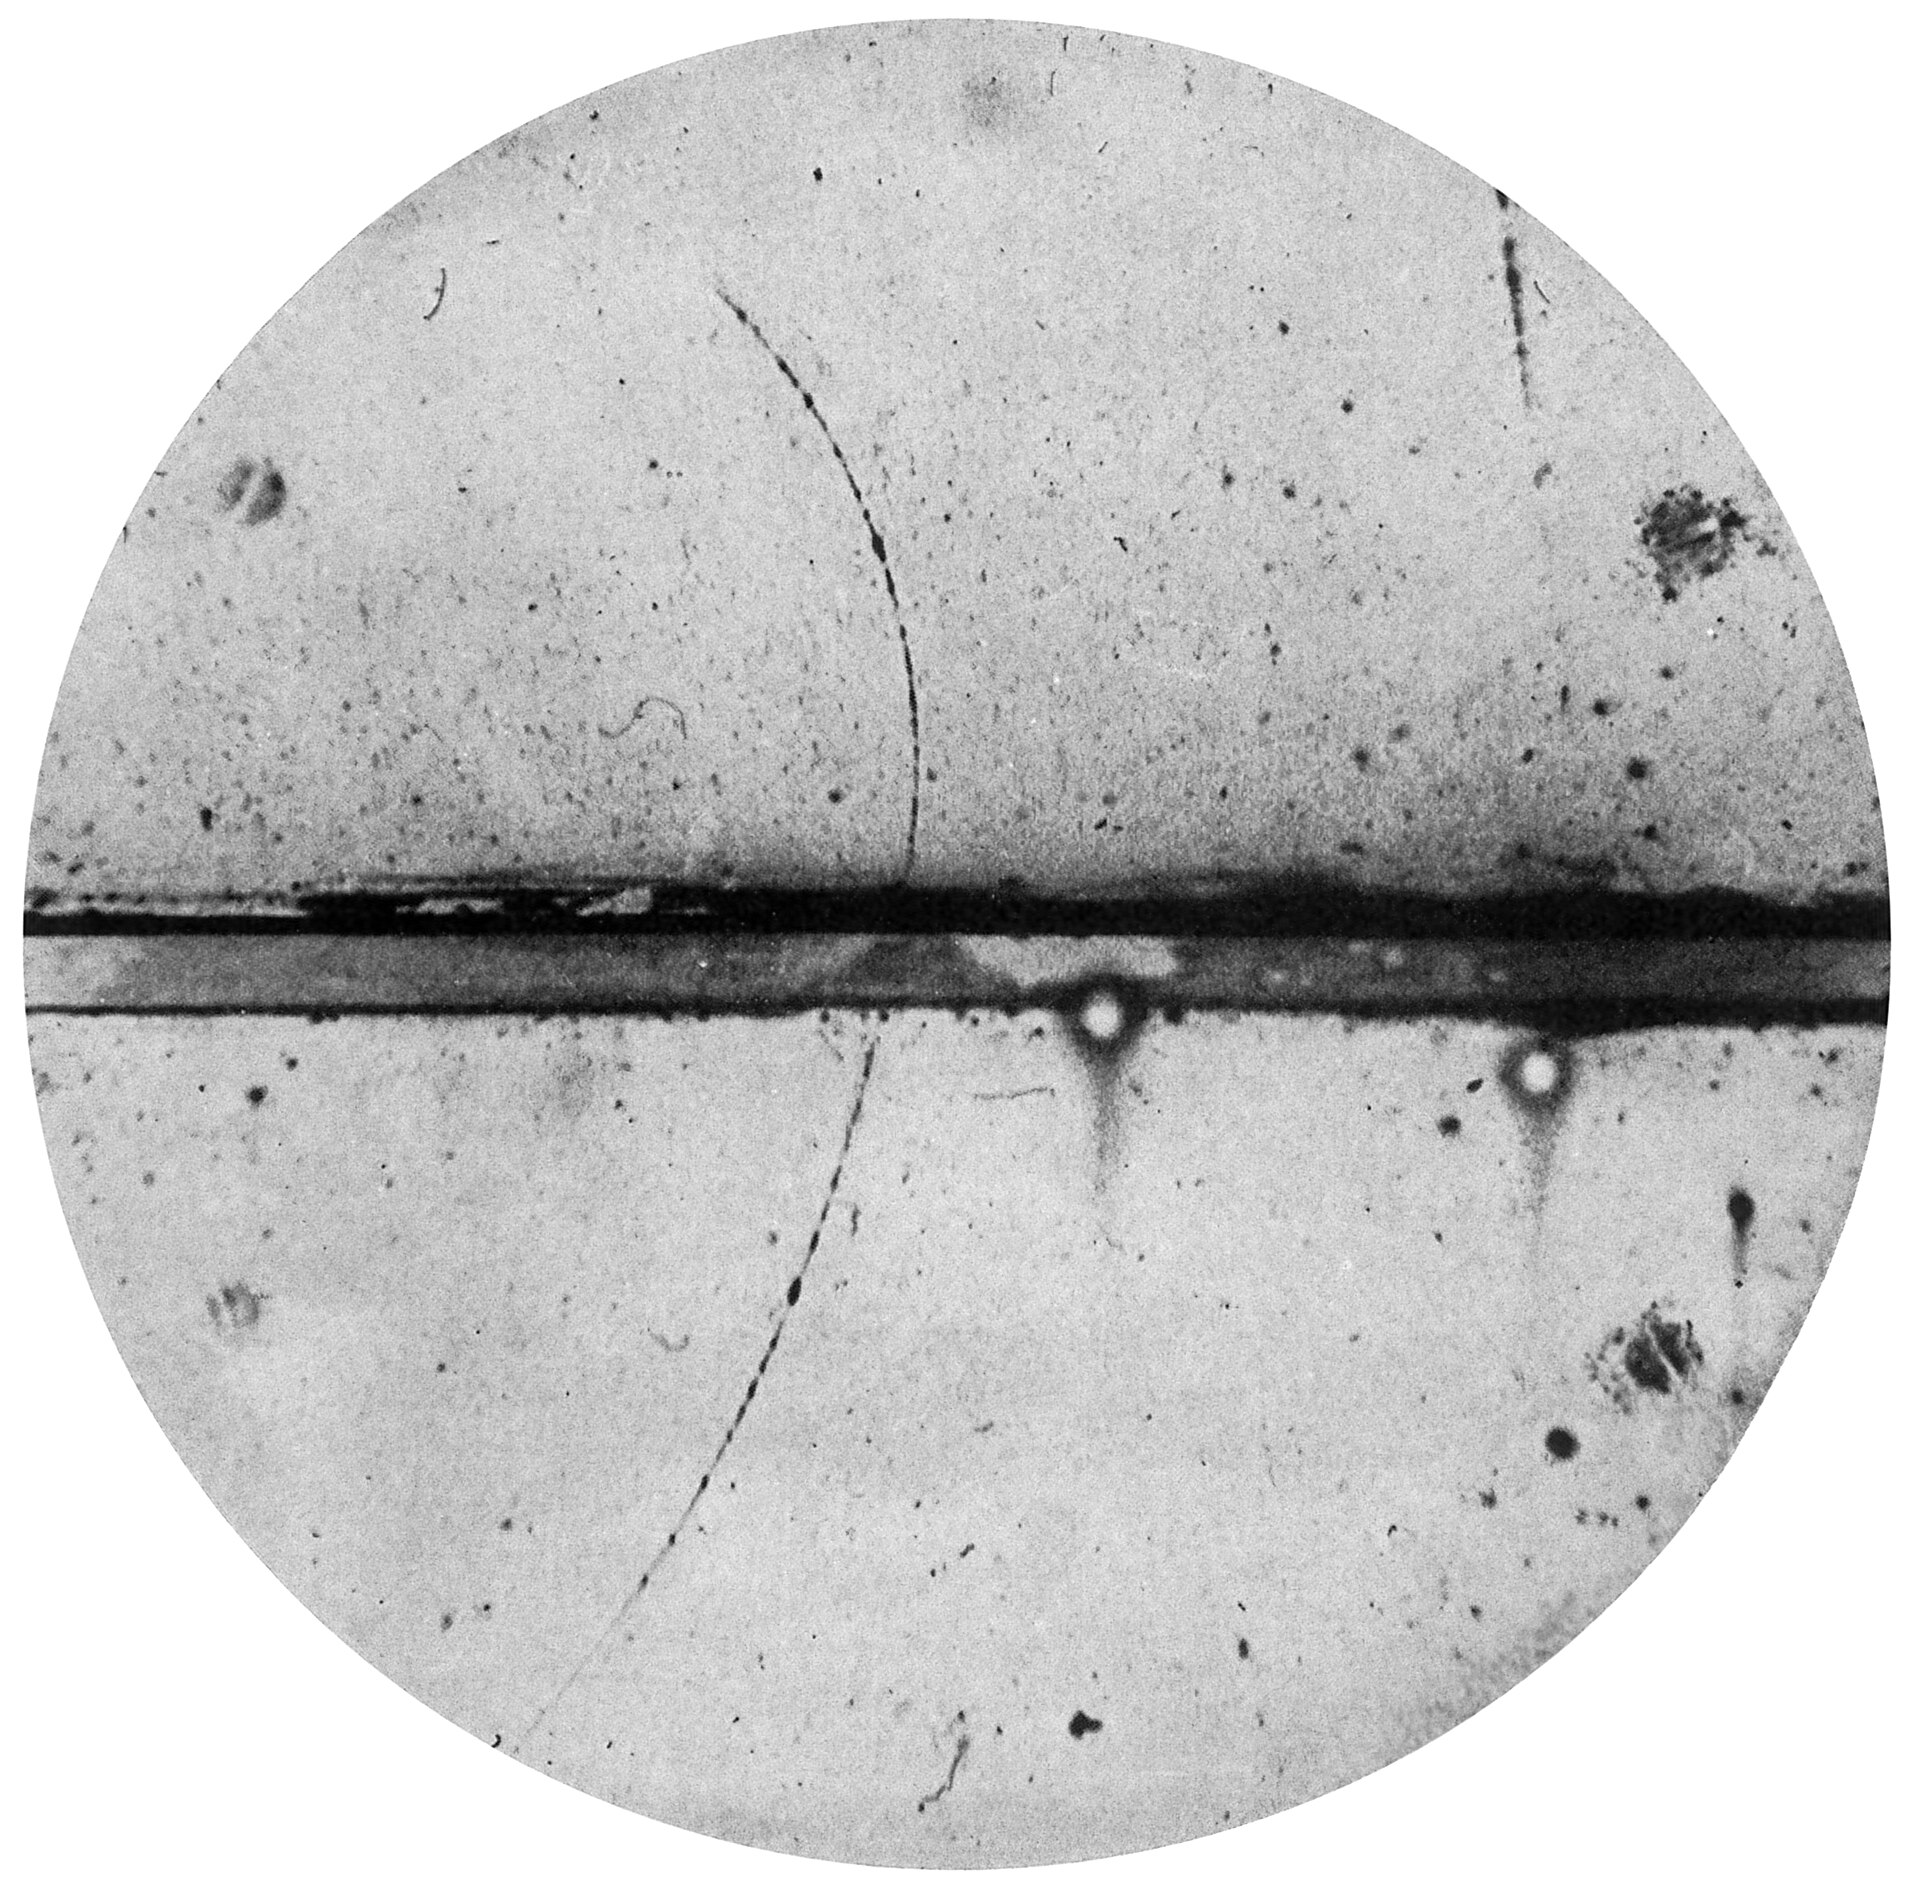
\includegraphics[width=0.5\linewidth]{images/book5/photo-positron-anderson.jpg}

{\small The discovery of antimatter (Carl D. Anderson, 1932, public domain): a single positron climbing through the cloud chamber's lead plate, curving the wrong way for an electron and too tightly for a proton --- $E = mc^2$'s ledger caught running in reverse.}
\end{omfigure}

\section{Problem: Making matter --- the antiproton and the Bevatron}

\begin{problem}[{Weekend problem --- how momentum conservation
priced the antiworld}]\label{pb:b3:relativistic-dynamics:1}
Dirac's equations demanded, from 1931, that the proton have a mirror
twin of opposite charge. Making one meant buying its \omterm{def:b3:relativistic-dynamics:momentum-energy}{rest energy} with
beam energy --- and momentum conservation set the price. This problem
prices it, designs the machine that paid it, and follows the 1955
discovery. Data: $m_{\text{p}}c^2 = \qty{938.3}{MeV}$; charge and
\emph{baryon number} (protons and neutrons $+1$, antiprotons $-1$)
are conserved in every reaction.

\medskip\noindent\textbf{Part I --- The \omterm{def:b3:relativistic-dynamics:four-momentum}{four-momentum} toolkit.}
\begin{enumerate}
  \item For one particle, show $E^2 - p^2c^2 = m^2c^4$ from the
        definitions of $E$ and $\vect p$.
  \item For a system, why is $E_{\text{tot}}^2 -
        p_{\text{tot}}^2c^2$ the same in all frames, and what does it
        equal in the centre-of-momentum frame?
  \item A proton beam of energy $E$ hits a proton at rest: show
        $M^2c^4 = 2m_{\text{p}}^2c^4 + 2E\,m_{\text{p}}c^2$.
  \item Check the two limits: at low energy $Mc^2 \to
        2m_{\text{p}}c^2$; at high energy $Mc^2 \approx
        \sqrt{2E\,m_{\text{p}}c^2}$ --- the square-root law.
  \item A reaction is allowed only if $Mc^2$ reaches the summed rest
        masses of the products, with all products at rest in the
        centre-of-momentum frame at threshold: justify this last
        clause.
  \item Why can the kinetic energy of the products in the lab never
        be recovered for particle creation on a fixed target?
\end{enumerate}

\medskip\noindent\textbf{Part II --- Pricing the antiproton.}
\begin{enumerate}[resume]
  \item In $p + p$ collisions, the cheapest reaction making an
        antiproton $\bar p$ must also make an \emph{extra} proton:
        write it, and justify with charge and baryon number.
  \item Show the threshold requires $Mc^2 = 4m_{\text{p}}c^2$.
  \item Deduce the required beam energy $E = 7m_{\text{p}}c^2$ and
        kinetic energy $T = 6m_{\text{p}}c^2$; evaluate $T$.
  \item At threshold, what fraction of the beam's kinetic energy
        actually became new rest mass ($2m_{\text{p}}c^2$ of it)?
        Where is the rest?
  \item In a head-on $p$--$p$ collider, what kinetic energy
        \emph{per beam} would the same reaction need? Compare the
        two designs.
  \item In 1954 no collider existed (beams were too thin to hit each
        other): what practical fact forced the fixed-target choice,
        and what did it cost in beam energy?
\end{enumerate}

\medskip\noindent\textbf{Part III --- Designing the Bevatron.}
The machine built at Berkeley reached $T = \qty{6.2}{GeV}$ ---
comfortably above threshold --- with dipole fields of $B =
\qty{1.56}{T}$.
\begin{enumerate}[resume]
  \item Compute the beam's total energy and momentum at top energy.
  \item Compute the bending radius $r = p/qB$ and compare with the
        machine's \qty{15.2}{m}.
  \item Compute the proton's speed and the revolution frequency on
        the $2\pi r$ ring.
  \item At injection the protons arrive at \qty{10}{MeV} kinetic:
        compute their speed, and explain why the accelerating
        frequency had to \emph{sweep} during each cycle (which two
        quantities change as $E$ grows?).
  \item With about \qty{1.5}{kV} gained per turn, how many turns and
        how long does one acceleration cycle take?
  \item The name ``Bevatron'' came from BeV, billions of
        electronvolts: state in one line what physics fixed the
        design figure of $6$ and a fraction BeV.
\end{enumerate}

\medskip\noindent\textbf{Part IV --- The discovery, 1955.}
\begin{enumerate}[resume]
  \item A magnet bends each candidate on a circle: explain why this
        selects particles by \emph{momentum} ($r = p/qB$), not by
        energy or speed --- and why a momentum-selected beam still
        mixes species.
  \item The beam on a copper target produced torrents of negative
        pions ($m_\pi c^2 = \qty{139.6}{MeV}$) among which a few
        antiprotons hid. The spectrometer selected negatives of
        momentum $p = \qty{1.19}{GeV}/c$: compute the speed of an
        antiproton and of a pion at that momentum.
  \item Over the \qty{12}{m} flight path, compute the two times of
        flight: what time resolution did the discovery need?
  \item A second, independent signature used \v Cerenkov counters,
        firing only above a speed threshold: which particle was
        arranged to fire it, and why does redundancy matter for a
        discovery?
  \item Chamberlain and Segr\`e counted about one antiproton per
        $\num{44000}$ pions: why did the threshold argument
        guarantee the rate would be tiny even above threshold?
  \item An antiproton eventually meets a proton and annihilates:
        how much energy is released per event, and into what,
        typically?
  \item Summarise the named result: conservation of \omterm{def:b3:relativistic-dynamics:four-momentum}{four-momentum}
        priced the antiproton at $T = 6m_{\text{p}}c^2 =
        \qty{5.6}{GeV}$ on a fixed target; a \qty{6.2}{GeV},
        \qty{15}{m} synchrotron paid it, and the antiworld became
        laboratory fact --- the Nobel Prize of 1959.
\end{enumerate}
\end{problem}
